\section{Dynamic VPNs} % (fold)
\label{sec:dvpns}

In Section~\ref{sub:scope} we already gave a short description of \acp{dvpn}. In this section, we will further look at the actual concept. Starting with defining what it actually provides, how it's carried over the core, the information needed to implement a \ac{vpn}, from where that information is available and finally working towards a list of technical requirements that the network will need to provide.

\subsection{Service} % (fold)
\label{sub:service}

To define the \ac{dvpn} service, we first take a look at the concepts of non-dynamic, or static \acp{vpn}. They can be classified depending on the \acs{osi} layer which it virtualizes, the protocol that is being used and the visibility to the customer. In an IPSec \ac{vpn} for example, the customer needs to setup his \acp{ce} at each site to actually establish the Layer 3 \acs{ip} \ac{vpn}. As we have already established in Section~\ref{sub:scope}, we limit the use-case to an multi-point Ethernet Layer 2 \ac{vpn} which is provisioned by the provider (\acs{ppvpn}) and thus requires no action on the \ac{ce}. Throughout this paper the definition of \ac{ppvpn} related terms will be used as described in RFC 4026 \cite{vpn-terms} and an overview is given in Figure~\ref{fig:ppvpn}.

What a Layer 2 \ac{ppvpn} provides to the \ac{ce} is a transparent connection to one or more other \acp{ce} using a single Ethernet broadcast domain. Another term to describe such a \ac{vpn} service is a \ac{vpls}. It enables the interconnect of several \acs{lan} segments over a seemingly invisible carrier network. To do so, the \ac{pe} needs to keep the \acp{cmac} ahead of the frame intact and also support the forwarding of broadcast and multicast traffic. All \acp{pe} (and of course \acp{p}) will not be visible to the \ac{ce}, who will regard the other \acp{ce} as part of the \ac{vpls} as direct neighbors on the network as illustrated in Figure~\ref{fig:ppvpn-cust}. 

\begin{figure}[!h]
	\centering
	\begin{subfigure}[h]{0.45\textwidth}
	\centering
		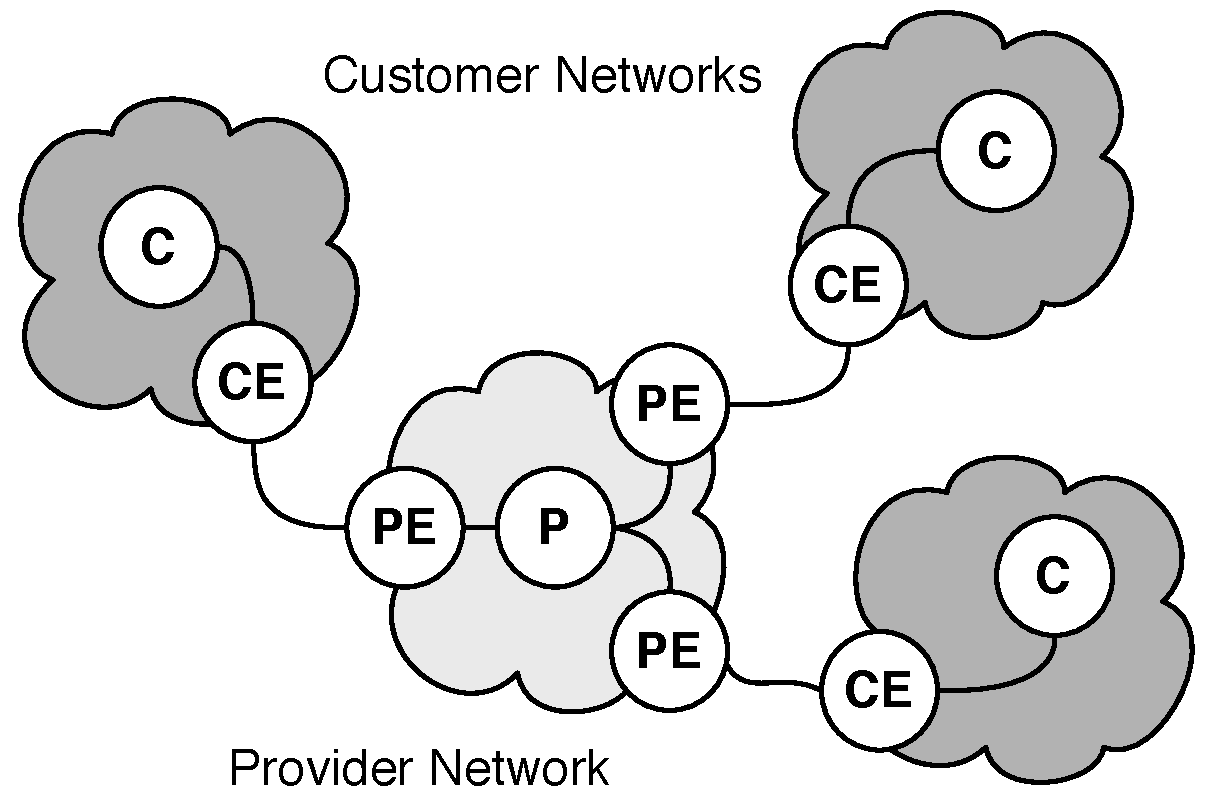
\includegraphics[width=\textwidth]{./includes/ppvpn.pdf}
		\caption{Terminology used to describe \acs{ppvpn} devices.}
		\label{fig:ppvpn}
	\end{subfigure}\hfill
	\begin{subfigure}[h]{0.45\textwidth}
	\centering
		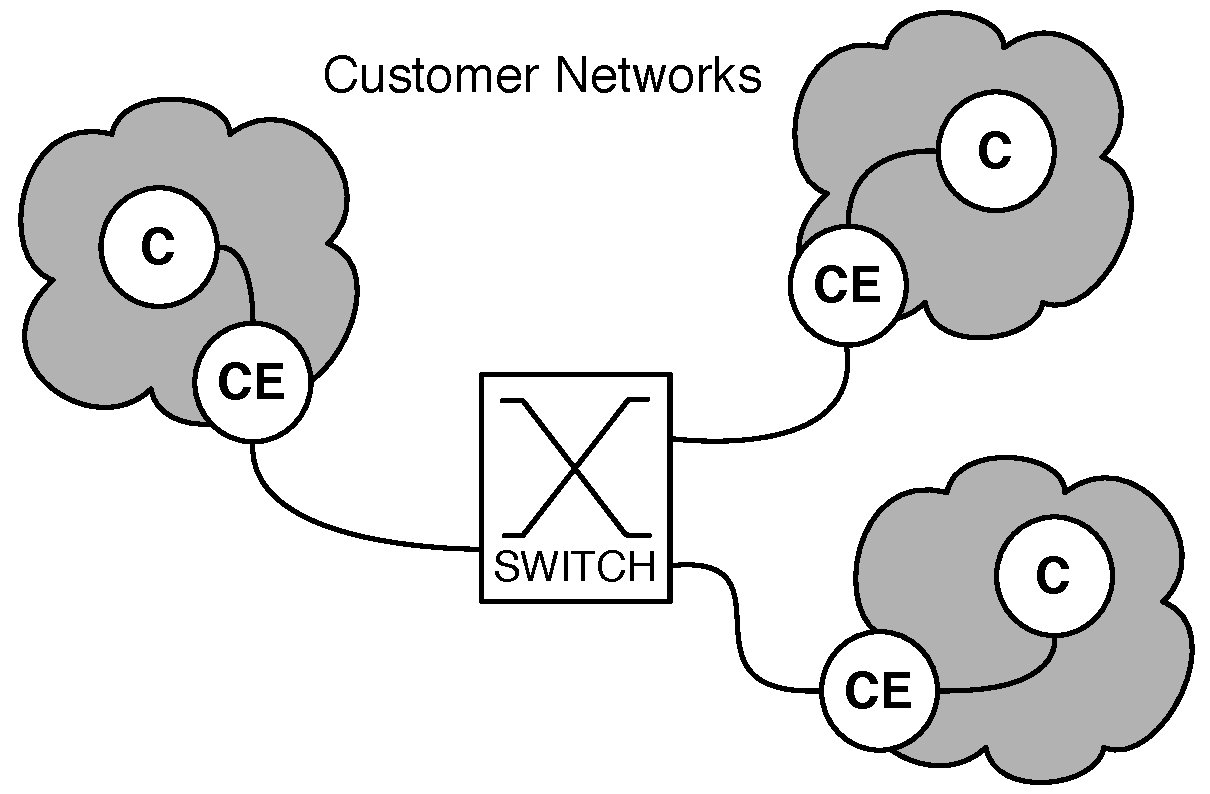
\includegraphics[width=\textwidth]{./includes/ppvpn-cust.pdf}
		\caption{Appearance of \acs{vpls} from customer point-of-view.}
		\label{fig:ppvpn-cust}
	\end{subfigure}
	\caption{Visualization of used terminology.}
\end{figure}

All these functionalities apply to \acp{vpn} as well as \acp{dvpn}. \acp{dvpn} however, also are flexible in nature. They can be configured, adapted and deconfigured within relatively short timespans. Current Layer 2 \acp{vpn} are mostly configured statically and changes in their configurations will require manual labor from the engineers. To convert them to \acp{dvpn} new tools are needed to automate this provisioning process which we will get back to in Section~\ref{sub:provisioning}.

% subsection service (end)

\subsection{Transport} % (fold)
\label{sub:transport}

Transporting a Layer 2 frame between two \acp{ce} starts at the \ac{pe}. The ingress \ac{pe} learns the \ac{sa} of the frame behind the port connected to the \ac{ce}, then it needs to forward the frame to the \ac{pe} where the \ac{da} is present. It will need to do so while separating the traffic from other \acp{dvpn}, it has to make the traffic unique and identifiable from the rest of the \acp{vpn} transported over the network. This is done by giving the frame some sort of `color' or `tag' specific to the customer \ac{vpn}. Additionally it should presume the that \ac{p} devices are not aware of the \ac{dvpn} and do not learn the \ac{cmac} addresses. This is because the network will have to scale to thousands of \acp{dvpn} and possibly millions of \acp{cmac} divided over those \acp{dvpn}. To provide this so called \acs{mac} Scalability, only \acp{pe} should learn the \acp{cmac}.

Forwarding from ingress \ac{pe} to egress \ac{pe} happens over a path of several \acp{p}. Every \ac{pe} connected to a \ac{ce} member of a particular \ac{dvpn}, should have one or more paths available to each and every other \ac{pe} with members of that \ac{dvpn}. The determination of the routes of these paths takes place through a form topology discovery. This mechanism should dynamically find all available \acp{pe} and \acp{p} with all the connections between them and allow for the creation of paths which are not susceptible to infinite loops.

The links comprising the paths have a certain capacity which will need to be used as efficiently as possible. This means that the links comprising a path will need to have enough resources available, but that other links need not be left vacant. Also, if the required bandwidth for a \ac{dvpn} exceeds the maximum capacity of one or more of the links in a single path, a second path should be installed to share the load towards the egress \ac{pe}. 

Continuing with the processing of the ingress customer frame, when it arrives at the ingress \ac{pe} with a \ac{da} unknown to the \ac{pe}, the frame will be flooded to all participating \acp{pe}. Upon arrival there, the egress \ac{pe} stores the mapping of the frames \ac{sa} to the ingress \ac{pe} and if it knows the \ac{da} will forward out the appropriate port. Because this is a virtual broadcast domain, all \ac{bum} traffic will need to be flooded to the participating \acp{pe}. To limit the amount of \ac{bum} traffic in a single \ac{dvpn} rate limits or filters will need to be in place to prevent the \ac{dvpn} from being flooded with it.

Another addition to rate limiting unknown unicast traffic is by pre-populating the \acs{mac} tables of the \acp{pe}. This requires that, besides the ingress \ac{pe} only learning the \ac{sa} from the \ac{ce}, it will also actively distribute the \ac{sa} to all other \acp{pe} with members of the same \ac{dvpn}. Then, instead of flooding unknown unicast frames to the \acp{pe}, the ingress \ac{pe} drops the frame, knowing that the other \acp{pe} will not recognize it either. This can also be extended to limit broadcast \ac{arp} traffic if the \acp{pe} also exchange the \ac{ip} address belonging to each \ac{cmac}. When the ingress \ac{pe} receives an \acs{arp} request for a certain \ac{ip} address, it can look it up in its table and without flooding the frame, reply to the \ac{ce} with the correct \ac{mac}.

\begin{figure}[!h]
	\centering
	\begin{subfigure}[b]{0.3\textwidth}
		\centering
		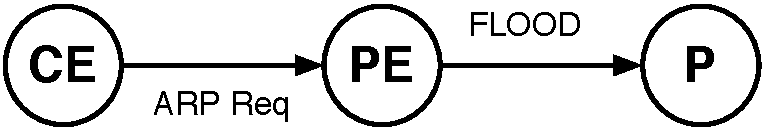
\includegraphics[width=\textwidth]{./includes/arp-no-proxy.pdf}
		\caption{Normal \acs{arp} Request.}
		\label{fig:arp-no-proxy}
	\end{subfigure}\hspace*{1cm}
	\begin{subfigure}[b]{0.3\textwidth}
	\centering
		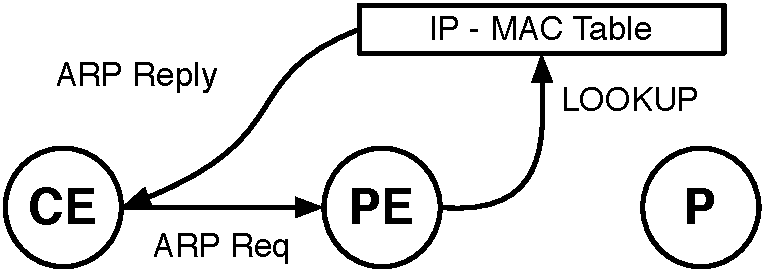
\includegraphics[width=\textwidth]{./includes/arp-proxy.pdf}
		\caption{\acs{arp} proxy in \ac{pe}.}
		\label{fig:arp-proxy}
	\end{subfigure}
	\caption{Processing of \acs{arp} requests at the \ac{pe}.}
\end{figure}

With multiple \acp{dvpn} present on the network it can happen that one \ac{dvpn} affects the available bandwidth of others. Therefor rate limits will need to be in place for the overall traffic coming in to the \ac{ce}-connected ports. Policing rates of different \acp{dvpn} in the core is nearly impossible, the hardware cannot police traffic of separate \acp{dvpn}. And, because it burdens the core with another responsibility while it should only be concerned with fast forwarding, is also undesirable. However, by assigning a minimum and maximum bandwidth rate to each \ac{dvpn} instance, it is possible to preprovision the paths over the network according to the required bandwidth. By also monitoring the utilization of individual links, \ac{dvpn} paths can be moved away from over-provisioned links while they are in use. However, the impact on traffic when performing such a switch must be minimized and should ideally last no longer than 50 ms.

To monitor and troubleshoot large carrier networks \ac{oam} functionalities need to be supported by the network. Monitoring end-to-end activity needs to available through automatic continuity check messages, but also by supporting `traceroutes' through the network manually. This enables the network react proactively to network failures by using a similar method as presented above when switching \acp{dvpn} to a different path, also known as `fast failover.'

% subsection transport (end)


\subsection{Provisioning} % (fold)
\label{sub:provisioning}

Before implementing a \ac{dvpn} in the network, the network first has to become converged. Meaning that the topology of the complete network is known and that paths can be created over this topology. 

A \ac{dvpn} instance consists of multiple member ports, which are identified by their \ac{pe} device and the port on that \ac{pe}. The instance also contains values for its minimum and maximum available bandwidth which can be used to determine the paths that the \ac{dvpn} will get assigned. When member ports reside on different \acp{pe}, a bidirectional path will need to be created through the network. The route of the path will depend on 
\begin{inparaenum}[\itshape a\upshape)]
	\item the liveness and administative availability of the links, 
	\item the administrative costs of the links, and 
	\item the resources available on the links towards the \ac{pe}.
\end{inparaenum}
The exact algorithm used to choose the paths lies outside of the scope of this document. Paths are defined by the physical ports that they traverse through the network, with the \acp{pe} as the first or last in the list.

When the path between two \acp{pe} has been setup for the \ac{dvpn}, it can be put in the \ac{dvpn} description. More paths may be added over different routes and paths may be adjusted during the lifetime of the \ac{dvpn}. This may for example be necessary when a certain link in the path fails, or when it nears its peak capacity and has to be rerouted. A simplified but complete information base diagram has been given in Figure~\ref{fig:infobase}. Individual port utilization will be monitored and when a certain link shows high utilization, the corresponding paths and \acp{dvpn} using those paths can be looked up using the information base. Also other monitoring and troubleshooting processes will profit from this information.

\begin{figure}[!h]
	\centering
	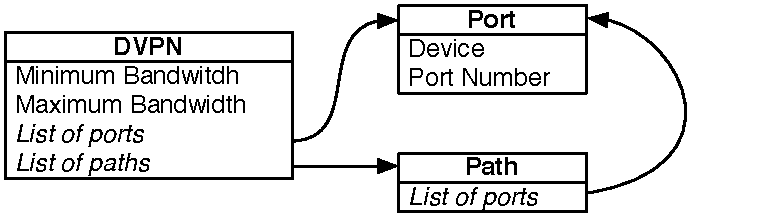
\includegraphics[width=10cm]{./includes/infobase.pdf}
	\caption{Information base of a \ac{dvpn}.}
	\label{fig:infobase}
\end{figure}

After the complete paths between \acp{pe} with \ac{dvpn} members have been setup the traffic can start flowing. However, as has been mentioned before, the rate limiting feature will need to be applied to the ingress ports to prevent the \ac{dvpn} from using up all the networks resources. 


% subsection provisioning (end)

\subsection{Requirements} % (fold)
\label{sub:requirements}


To summarize, to be qualified to deploy \acp{dvpn}, networking technologies will need to be able to provide the following features:

\begin{enumerate}
	\item identify traffic from separate \acp{dvpn} by tagging, 
	\item scalable up to thousands of \acp{dvpn} and \acsp{cmac},
	\item topology discovery, 
	\item provision paths over the network,
	\item efficient use of, and control over all network resources (\ac{te}),
	\item share the load of traffic over multiple paths,
	\item rate limiting or filtering of \ac{bum} traffic,
	\item rate limiting of total \ac{dvpn} traffic per port,
	\item fast failover times (<50ms) to provide continuity to critical applications,
	\item provide \acl{oam} features to monitor and troubleshoot the network.
\end{enumerate}

Besides the forwarding specific requirements the provisioning system will also need to be able to:

\begin{enumerate}
	\item take input as certain ports to be placed in a \ac{dvpn},
	\item determine routes that can be used for the paths,
	\item monitor links and reroute paths on failure or peak capacity,
	\item set the rate limits on ingress \ac{pe} ports.
\end{enumerate}

% subsection requirements (end)

% section dynamic_vpns (end)